%
% File naacl2019.tex
%
%% Based on the style files for ACL 2018 and NAACL 2018, which were
%% Based on the style files for ACL-2015, with some improvements
%%  taken from the NAACL-2016 style
%% Based on the style files for ACL-2014, which were, in turn,
%% based on ACL-2013, ACL-2012, ACL-2011, ACL-2010, ACL-IJCNLP-2009,
%% EACL-2009, IJCNLP-2008...
%% Based on the style files for EACL 2006 by 
%%e.agirre@ehu.es or Sergi.Balari@uab.es
%% and that of ACL 08 by Joakim Nivre and Noah Smith

\documentclass[11pt]{article}
\usepackage[hyperref]{naaclhlt2019}
\usepackage{times}
\usepackage{latexsym}
\usepackage{tikz,pgf}
\usetikzlibrary{arrows}
\usepackage{verbatim}

\usepackage{url}

\aclfinalcopy % Uncomment this line for the final submission
%\def\aclpaperid{***} %  Enter the acl Paper ID here

%\setlength\titlebox{5cm}
% You can expand the titlebox if you need extra space
% to show all the authors. Please do not make the titlebox
% smaller than 5cm (the original size); we will check this
% in the camera-ready version and ask you to change it back.

\newcommand\BibTeX{B{\sc ib}\TeX}

\title{Document Reconstruction from a Bag of Tokens using Trigrams and 5-grams from a Corpus of Related Documents}

\author{Brad Burkman \\
  University of Louisiana at Lafayette \\
  Louisiana School for Math, Science, and the Arts \\
  {\tt bburkman@lsmsa.edu} 
 }

\begin{document}
\maketitle

%%%%%%%%%%
\begin{abstract}
	We have a bag of tokens, perhaps from a corrupted document, and a corpus of documents known (or supposed) to be ``similar'' to the original document.  Can we use the corpus to reconstruct a ``best guess'' approximation of the original document?
	
	We propose a new method.  We first use the word frequencies in the corpus to order the bag of tokens and turn it into a bag of words with a Ziphian distribution.  Then we make a graph from the corpus trigrams and find a path through the graph that links tokens to build a string of words to form a candidate document.  
	
	We have scored the candidate using two metrics and plan to add a third:  (a) the sum of the corpus frequencies of the trigrams in the path, (b) the sum of the frequencies of any corpus 5-grams that appear in the candidate document, and (c, not yet implemented) a measure of how closely the word distribution in the candidate document approximates the Zipfian distribution of the bag of words.
	
	In development we used the NLTK {\tt Inaugural} corpus, the texts of fifty-six US Presidential Inaugural Addresses \cite{Bird:09}.  We plan to also test it on other corpuses.   
	
	We discuss why we believe our method, while it may be interesting, is not likely to be successful as currently envisioned.  
	
\end{abstract}

%%%%%%%%%%%
\section{Credits}

This paper is a project for CSCE 561, Information Storage and Retrieval, taught by Dr. Aminul Islam at the University of Louisiana at Lafayette.  

The code relies on NLTK, the Natural Language Toolkit \cite{Bird:09}, and \verb|graph-tool| \cite{peixoto_graph-tool_2014}.

%%%%%%%%%%%%%
\section{Introduction}

The goal of Natural Language Generation (NLG) is to build sentences (which are subsequently built into conversations or documents) from some information stored in a structured form \cite{Matulik:18}, and it is hard.  Even small improvements are important \cite{Barros:15}.

The algorithms for Natural Language Generation are $np$-hard with $O(n!)$ because we have to consider all (or most) possible paths through the graph.  If we find all walks with unlimited cycles, even in a small graph, then we have an $O(\infty)$ problem.  In many other related problems we could prune branches early when we realized that the path was not going to lead to an optimial outcome, but NLG is like the game of Go, that `` their outputs can be evaluated
only when their process reaches the last state'' \cite{Kumagai:16}.

The hypothetical application considered here is that we have a corpus of ``similar'' documents, and there is another similar document for which we only have a bag of tokens.  Our goal is to find a ``best'' candidate for a reconstruction of the lost document using the corpus.  

We chose to work with the NLTK Inaugural corpus, and from that generated a smaller bag of tokens from the tokens in the corpus.  Following the method described below, we applied a corpus-derived Zipfian frequency distribution to turn the bag of tokens into a bag of words and worked towards generating a candidate reconstruction of the ``lost'' document by finding and scoring paths through the graph of trigrams.  

\section{Original Contributions}

We believe that our scoring mechanism is novel and useful.  While we have only implemented the first two stages, we believe that this set of three metrics would give a good measure of similarity to our goal, finding the candidate that most closely represents both the bag of words and the phrasing of the corpus documents.  

The first metric is the corpus frequency of the trigrams used in the candidate document.  Since the candidate is constructed by linking corpus trigrams, this metric will be at least the number of trigrams in the candidate, but will favor candidates that use trigrams more common in the corpus.  

The second metric is the corpus frequency of the corpus 5-grams that appear in the corpus.  The algorithm constructs the candidates with no reference to the 5-grams, but since 5-grams reveal longer phrases than trigrams, this metric will give a better measure of how close the candidate is to the grammatical and oratorical patterns of the corpus.  

The third metric will be the similarity between the word frequency distribution in the candidate and the bag of words.  

Adding more metrics like 7-grams would push the candidates towards splicing together long phrases from individual speeches rather than taking the corpus as a whole.  Also, in a corpus this small (fifty-six documents), it is unlikely that many 7-grams would have a document frequency more than one. 

We believe that these three metrics together give a better measure than any of them separately.  Given that we have no gold standard for evaluating the quality of the candidates, this set of metrics may be among the best options.  

%%%%%%%%%%%%%%
\section{Related Work}

Other work has similarly tried to build new texts word-by-word by choosing a few starting words and analyzing a corpus to see which words could follow those, building up the text iteratively.  Matulik did this with a probabilistic model \cite{Matulik:18}.  Srivastava built up a document letter by letter, based on the previous hundred letters \cite{Srivastava:18}.

Baptiste Fontaine, a contributor to Homebrew and other projects, has a trigrams-based random text generator on GitHub \cite{Fontaine:14}.  It takes in some texts and returns a text, by default up to seventy words.  The documentation does not indicate the method or whether there is a scoring mechanism.  

%%%%%%%%%%
\section{Method}

In development we used as the corpus of documents the {\it C-Span Inaugural Address Corpus}, fifty-six speeches available in NLTK as {\tt Inaugural} \cite{Bird:09}.  



We will illustrate the methods with results from a run on eight of the speeches.  More than eight speeches made the $O(n!)$ path calculations unreasonably long for this stage of the project.  

\begin{figure}[h]
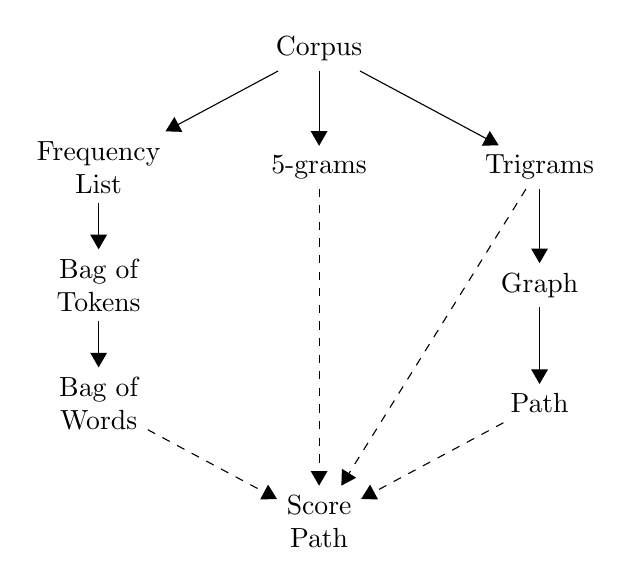
\begin{tikzpicture}[x=28mm,y=15mm]
	\node (A) at (0,0) {Corpus};
	\node (B) [align=center] at (-1,-1) {Frequency \\ List};
	\node (C) at (0,-1) {5-grams};
	\node (D) at (1,-1) {Trigrams};
	\node (E) [align=center] at (-1,-2) {Bag of \\ Tokens};
	\node (F) [align=center] at (-1,-3) {Bag of \\ Words};
	\node (G) [align=center] at (1,-2) {Graph};
	\node (H) [align=center] at (1,-3) {Path};
	\node (I) [align=center] at (0,-4) {Score \\ Path};
	\draw [-triangle 60] (A) -- (B);
	\draw [-triangle 60] (A) -- (C);
	\draw [-triangle 60] (A) -- (D);
	\draw [-triangle 60] (B) -- (E);
	\draw [-triangle 60] (E) -- (F);
	\draw [-triangle 60] (D) -- (G);
	\draw [-triangle 60] (G) -- (H);
	\draw [-triangle 60, dashed] (F) -- (I);
	\draw [-triangle 60, dashed] (C) -- (I);
	\draw [-triangle 60, dashed] (D) -- (I);
	\draw [-triangle 60, dashed] (H) -- (I);
	
\end{tikzpicture}
\caption{Simplified Overview of the Method}
\end{figure}

\subsection{Create a ``Similar'' Bag of Tokens}

First, create a corpus bag of words with document and frequency counts.  

\vskip 6pt
\begin{tabular}{rrl}
56 &9281& the \cr
56 &6970& of\cr
56 &6840& ,\cr
56 &4991& and\cr
56 &4676& .\cr
& $\vdots$ & \cr
1& 1& medicine\cr
1& 1& chattel\cr
1& 1& blueprint\cr
\end{tabular}
\vskip 6pt

Second, cull the list.  We chose to eliminate any words appearing in fewer than five of the speeches.  Of the remaining words, we accepted any with a frequency over 1000, and randomly culled the rest with this test:

\noindent{\tt frequency > random.randint(1,1000)}

which prefers words with higher frequency but may accept some with lower frequencies.  

This culling left us with ninety-one words, which we took as the Bag of Tokens.  

\subsection{Zipfian Frequency Distribution}

We made a bag of words by ordering the bag of ninety-one tokens by corpus frequency and giving the list a Zipfian frequency distribution, using {\tt zipf = int(91/r)}, rounding down the quotient where $r$ is the word's rank.

\vskip 6pt
\begin{tabular}{rrl}
56& 91& the \cr
56& 45& of \cr
56& 30& , \cr
56& 22& and \cr
56& 18& . \cr
& $\vdots$ & \cr
6& 1& propose \cr
9& 1& borne\cr
6& 1& immediately\cr
\end{tabular}

\subsection{Trigrams}

Our goal is to collect all trigrams we can link together to make a candidate document.  Each useful trigram will contain only words in the bag of words, and it will be able to link to a preceding and following trigram.  Two trigrams link if the last two words of the first match the first two words of the second.  

We will use the corpus frequencies of the trigrams to score candidate documents.  We preserve capitalization and punctuation for syntax.

Collect the (13695) corpus trigrams, and cull all trigrams that contain a word not in the bag of words (cut to 525).   Then iteratively remove all trigrams that do not have both another trigram to precede and to follow (cut to 115).  

\vskip 6pt
\begin{tabular}{rl}
25& the United States\cr
22& , and the\cr
17& of the United\cr
13& . It is \cr
12& of the people\cr
12& fellow - citizens\cr
$\vdots$ \cr
\end{tabular}

\subsection{Big Missing Step}

We suspect we missed a big step here, that the culled set of trigrams does not contain some words in the bag of words.  What we need is a set of trigrams that contains all of the words in the bag and only the words in the bag.  If the trigrams do not contain almost all of the bag of words, there is no hope of constructing a good document from them.   We need to iteratively cull both the bag of words and the trigrams until the two lists converge.  Depending on the starting list of words, the sets may converge at two empty lists.  

\subsection{5-grams}

The role of the 5-grams is to score the candidate documents according to the corpus frequency of the 5-grams they contain.  Thus, we do not need to keep the 5-grams that contain words not in the bag of words, but the 5-grams do not need to link.  

We start with 14763 5-grams and reduce it to 751.  

\vskip 6pt
\begin{tabular}{rl}
4& of our fellow - citizens\cr
3& of the United States .\cr
3& the Constitution of the United\cr
3& Constitution of the United States\cr
3& of the United States ,\cr
$\vdots$\cr
\end{tabular}

\subsection{Graph of Trigrams}

The trigrams form a directed graph, probably cyclic.  Each trigram is a vertex, and there is a directed edge from trigrams $A$ to $B$ if the last two words in $A$ match the first two words in $B$, that is, if $B$ can follow $A$.  Our task of creating a candidate document is analogous to taking a walk through the graph.  We will limit the number of possibilities by only considering paths.  [A {\it path} is a walk in which no node appears more than once \cite{Wilson:90}.]

We used the python module {\tt graph-tool} to create the graph and find all of the paths, each of which forms a candidate document.  \cite{peixoto_graph-tool_2014}.  

\subsection{Candidate Scoring, with an Example}

The highest-scoring candidate document in our sample run had fifty-nine words.  

{\tt , and the rights , and to the rights and safety . I have , in the power of the law , and in its administration , and with it , and that of which the Constitution of the Constitution , which is in the other , that the safety with which we have not , it is in}

Those fifty-nine words came from these fifty-seven trigrams (with their corpus frequencies).
\vskip 6pt

\begin{tabular}{rl}
22& , and the\cr
1& and the rights\cr
1& the rights ,\cr
2& rights , and\cr
12& , and to\cr
$\vdots$&\cr
1& have not ,\cr
1& not , it\cr
4& , it is\cr
2& it is in\cr
\end{tabular}
\vskip 6pt

Summing the corpus frequencies gives a trigram score of 150.

The candidate contains these corpus 5-grams, and earns a 5-gram score of 7, giving a total candidate score of 157. 
\vskip 6pt
\begin{tabular}{rl}
1& in the power of the\cr
2& of the law , and\cr
1& in its administration , and\cr
1& , and with it ,\cr
1& the Constitution , which is\cr
1& have not , it is\cr
\end{tabular}
\vskip 6pt

%%%%%%%%%%%%%
\section{Ways to Improve this Approach}

\subsection{Measure Word Frequency Similarity}

We hope later to implement the third scoring metric, the similarity between the word frequency in the candidate and the Zipfian word frequency of the bag of words.  

\subsection{Give Heavy Weight to the 5-gram Metric}

The 5-gram metric gives the best insight into how well the candidate represents the corpus.  Giving it two or three times the weight of the trigram metric may be appropriate.  

\subsection{Walk v/s Trail v/s Path}

In the case of a directed graph like ours, a {\it walk} is a is a succession of edges connecting nodes.  If all of the edges are different, the walk is a {\it trail}.  If all of the nodes are different, then the trail is a {\it path}.  If the first and last node are the same, then the path is a {\it cycle}.  A cycle can become a path by removing the first or last edge.  \cite{Wilson:90}

In mining the graph, our code (at this stage) only scores paths.  It does look for cycles, but while it is possible that a cycle could score higher than a path, we have not seen it.  Also, in the context of a speech, the first word should start with a capital letter and the last should be final punctuation in \{ `.`, `?', `!' \}.  In such a document, the first and last trigrams would not overlap by two words; thus, a speech cannot be a cycle.  

We limited our search to paths, rather than general walks, because in our previous attempts and in others' work we had seen the search get stuck in a cycle, generating an endless repetitive speech.  It would score well, but not be good natural language generation.  

We should consider adding some flexibility.  Considering trails instead of paths would allow the same trigram to be used more than once, but not repeat cycles.  Adding flexibility could exponentially increase compute time, however, so finding a balance would be a challenge.  




%%%%%%%%%%%%
\section{Limitations of this Approach}

\subsection{No Gold Standard}

We had no gold standard against which to measure our ``best'' documents; furthermore, such a gold standard would be problematic to construct and difficult to implement.  Given a large corpus and a large bag of words (more than ten tokens), there would be many ways to make a ``good'' document.  Which is ``best''?  How would one measure how close a given candidate is to the ``best'' document, and how would one automate the evaluation?  The process would have so many layers of subjectivity that it would be difficult to create and implement.  

\subsection{Correct Path may not Exist}

To construct a perfect document from a bag of tokens using this method, we would need a set of corpus trigrams that contain only, and all of, the words in the bag of tokens.  Those trigrams would need to form a directed graph through which there is a path that hits each word in the bag of tokens exactly the number of times in the Zipfian frequency distribution in the bag of words.  

While it may be possible to artificially construct a bag of tokens for which there would be such a set of corpus trigrams forming a graph with such a path, it is not likely that an arbitrary bag of tokens from the corpus would have such a path, even a path with most of the bag of words, especially if the corpus were small.  

\subsection{Compute Time}

If the corpus were large, the corresponding trigram graph would also be large, and the cost of finding the longer paths is an $O(n!)$ problem.  To know that we have found the ``best'' path, we would have had to find and compared all of them.  The path may exist, but we could not find  in a reasonable amount of time.  

If the graph is not connected, which is not unlikely, the problem can be broken down into searches in connected subgraphs.  If the disconnected graph with $n$ nodes is formed by connected subgraphs with $p$, $q$, and $r$ vertices, then considering them separately reduces a problem of $O(n!)$ to $O(p!+q!+r!)$ with $n= p+q+r$.  

%%%%%%%%%%%
\section{Conclusion}

We believe that our set of three metrics is novel and useful.  Our approach of making the linked trigrams into a directed graph allows us to take advantage of existing optimized tools.  We need to further explore whether it is possible to make a set of corpus trigrams that contains all of, and only, the words in a bag of tokens.  It may be necessary to introduce some more degrees of freedom that will exponentially increase compute time.  Finding an appropriate balance will be the challenge.  

%%%%%%%%%%%
\section*{Acknowledgments}

I would like to acknowledge the help of Dr. Aminul Islam for his suggestions and ideas from his lectures, and of my colleague Jennifer Mangum for teaching me Graph Theory.  

%%%%%%%%%%%
\appendix
\section*{Code}

The code is available at \url{https://github.com/bburkman/CSCE_561/tree/master/NLG}.  The main function is in \verb|NLTK02_Start.py|.

%%%%%%%%%%%%%
\bibliography{naaclhlt2019}
\bibliographystyle{acl_natbib}


\end{document}
